\chapter{Versuchsaufbau}

\begin{figure}[H]
    \centering
    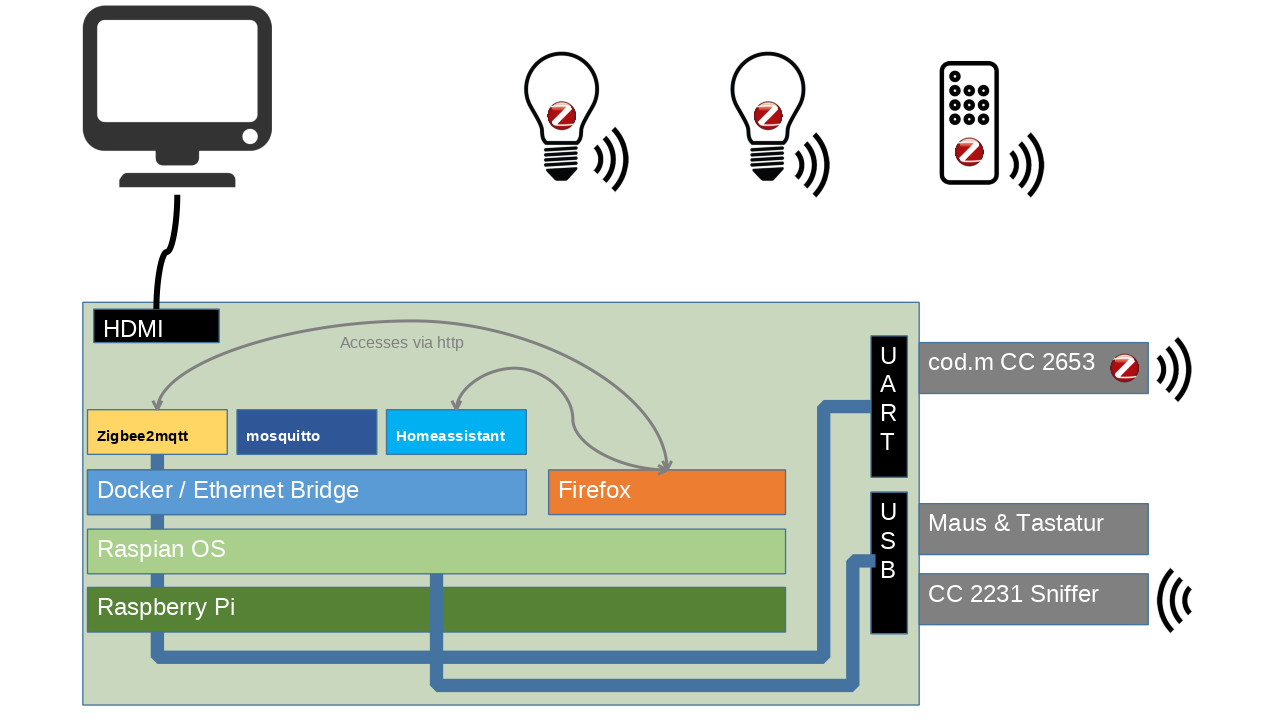
\includegraphics[width=1\textwidth]{media/Versuchsaufbau/image1.png}
    \caption{Versuchsaufbau}
  \end{figure}

In dieser Abbildung wird der schematische Versuchsaufbau gezeigt. Die drei Anwendungen werden als Docker Container gestartet. Sie kommunizieren
untereinander über eine eigenes Docker Netzwerk. Dies ist im eine von Docker verwaltete Linux Bridge. Nur der NGINX Reverse Proxy hat zwei Ports, die
auf die Host Interface gemappt werden. Die Wegfrontends sind damit über den lokal installierten Browser erreichbar. Damit ist der Raspberry Applikationsserver
und Versuchs-PC zugleich.

Die Hostnames werden in der lokalen hosts Datei angelegt, damit die Namen Lokal ausfgelöst werden.

Der cod.m Zigbee Hat wird direkt an den Docker Container durchgereicht. Der Sniffer Stick ist regulär am Host angeschlossen. 

\subsection{Containerverwaltung}

Die Container werden mit dem CLI Tool \grqq Docker-Compose \grqq{} verwaltet. Im folgenden werden die Definitionen der einzelnen Services erläutert.

\subsubsection{Nginx Proxy}
\begin{lstlisting}
    proxy:
      container_name: nginx
      image: jwilder/nginx-proxy:alpine
      networks:
        - backbone
      ports:
        - 80:80
        - 443:443
      volumes:
        - ./NGINX/proxy/conf.d:/etc/nginx/conf.d:rw
        - ./NGINX/proxy/vhost.d:/etc/nginx/vhost.d:rw
        - ./NGINX/proxy/html:/usr/share/nginx/html:rw
        - ./NGINX/proxy/certs:/etc/nginx/certs:ro
        - /etc/localtime:/etc/localtime:ro
        - /var/run/docker.sock:/tmp/docker.sock:ro
      restart: unless-stopped
\end{lstlisting}

Der Service Proxy basiert auf einem Image von des Reverse Proxys NGINX \cite{nginxpm}, erweitert durch \grqq jwilder \grqq{}. Vorteil dieses erweiterten Images ist es,
dass dieser automatisiert seine Konfigurationen anpasst. Zu diesem Zweck ist der \grqq docker.sock \grqq{} in den Container gemountet. Hierüber erfährt
der Proxy, ob Container gestartet worden sind, und welche Umgebungsvariablen gesetzt worden sind. Wird ein weiterer Container mit der Umgebungsvariable 
\grqq VIRTUAL\_HOST=z2m.local \grqq{} gestartet, wird automatisch eine Weiterleitung für alle Anfragen auf \grqq z2m.local\grqq{} eingerichtet auf den entsprechenden Container.
Dies erlaubt es beliebig viele Services auf einfache Art und weiße auf einem Host verfügbar zu machen. Zusätzlich sind alle Servicecontainer in einer 
eigenen L2-Domäne und sind von außen nicht erreichbar. Dies erhöht die Sicherheit, da Zugriff von außen nur über die beiden gemappten Ports des Proxys 
erfolgen kann. Dem Proxy wird daher entsprechend das Netzwerk 'backbone' zugewiesen. Im Abschnitt \grqq Ports \grqq{} können Ports nach außen gemappt werden.
In diesem Fall wird der Port 80 und 443 des Proxys auf die öffentlichen Ports 80 und 443 des Hosts gemappt. Hierfür werden von Docker Regeln in die 
\grqq iptables \grqq{} geschrieben. 

\begin{figure}[H]
  \centering
  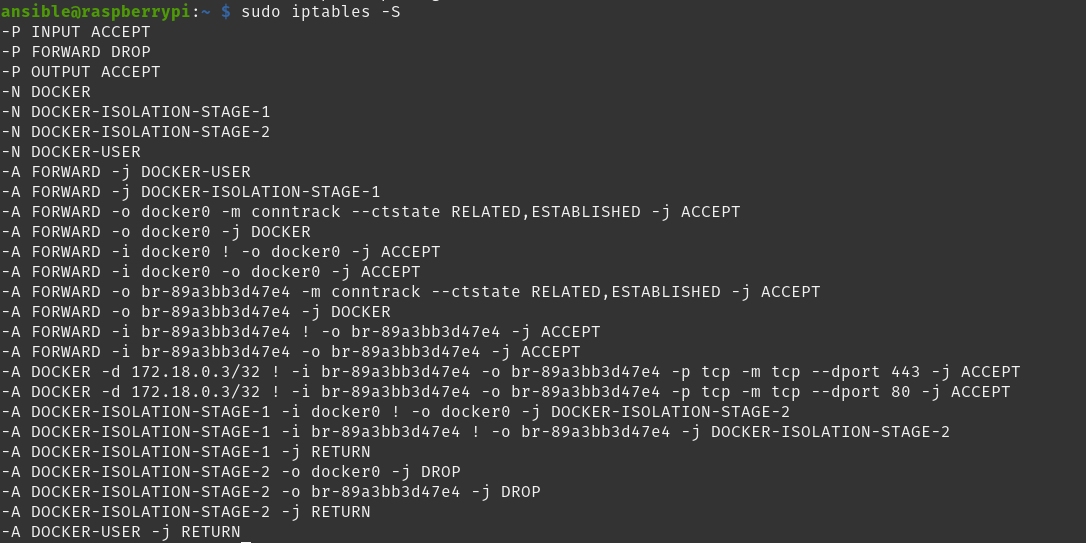
\includegraphics[width=1\textwidth]{media/rasp-iptables.png}
  \caption{Raspberry iptables}
\end{figure}

Die Regeln im Table \grqq DOCKER \grqq{} werden durch Docker geschrieben, diese sollen nicht modifiziert werden. Eigene Regeln können in den Table 
\grqq DOCKER-USER \grqq{} definiert werden.

\begin{figure}[H]
  \centering
  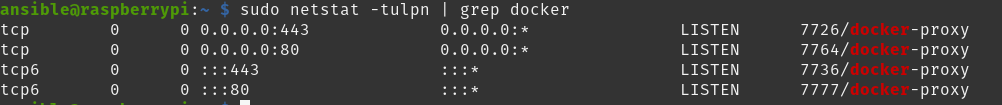
\includegraphics[width=1\textwidth]{media/rasp-netstat.png}
  \caption{Raspberry netstat}
\end{figure}

In diesem Output ist erkennbar, dass Docker einen Listener auf den Ports 80 und 443 laufen hat.

\subsubsection{zigbee2mqtt}
\begin{lstlisting}
  zigbee2mqtt:
  container_name: zigbee2mqtt
  image: koenkk/zigbee2mqtt
  networks:
    - backbone
  volumes:
    - ./Z2M/data:/app/data
#    devices:
    # CC251
    # - /dev/ttyUSB0:/dev/ttyACM0
    # CC2530 / GBAN GB2530S
    #- /dev/ttyUSB_cc2530:/dev/ttyACM0
  restart: always
  environment:
    - VIRTUAL_HOST=z2m.local
    - VIRTUAL_PORT=8080
  group_add:
    - dialout
\end{lstlisting}

Der Container wird ebenfalls an das Netzwerk \grqq Backbone \grqq{} angeschlossen. Der Ordner mit den Konfigurationen wird auf den Host gemountet und 
bleiben damit konsistent, auch wenn der Container als solches getauscht wird. Wenn der gemountete Pfad außerhalb des Containers nicht existiert, wird der 
Ordner aus dem Container gemountet. Exisitert der Pfad, wird der Ordner vom Host in den Container gemountet. Durch das Linux-Mantra \grqq Everything is a file \grqq{}
ist es auch möglich Geräte über die selbe Art und Weise in einen Container zu mounten wie einen regulären Dateipfad. **** ist der Socket zu dem cod.m Modul.
In den Umgebungsvariablen wird dem Proxy noch mitgeteilt, unter Welcher URL er erreichbar sein soll und auf welchem Port der Webserver läuft. Die Gruppe 
\grqq dialout \grqq{} ist notwendig, damit der Container Zugriffsrechte. Der Container Prozess läuft mit entsprechenden Rechten.

Im Playbook \grqq DeplayLabutils \grqq{} wird folgende Konfiguration eingespielt:
\begin{lstlisting}
  homeassistant: true
permit_join: false
mqtt:
  base_topic: zigbee2mqtt
  server: mqtt://mosquitto:1883
serial:
  port: /dev/ttyACM0
frontend:
  port: 8080
  host: 0.0.0.0
  url: https://z2m.local
advanced:
  homeassistant_legacy_entity_attributes: false
  legacy_api: false
  legacy_availability_payload: false
device_options:
  legacy: false
\end{lstlisting}

Es wird der Modus \grqq homeassistant \grqq{} aktiviert, damit werden die Nachrichten an den MQTT Broker so gestaltet, dass homeassistant diese versteht.
Das Beitreten neuer Geräte ist im Standard aus und muss explizit erlaubt werden. Desweiteren wird ein MQTT Server angegeben, sowie ein \grqq base-topic \grqq{}
definiert. Docker löst Containernamen in Dockernetzwerken auf zu IP-Adressen, sodass hier als server einfach der entsprechende Containernamen angegeben werden
kann. Im weiteren wird der Pfad angegeben, auf den der cod.m Adapter gemountet wurde, sowie entsprechende Einstellung für den Webserver gesetzt.

\subsubsection{mosquitto}

\begin{lstlisting}
  mosquitto:
  container_name: mosquitto
  image: eclipse-mosquitto:latest
  networks:
    - backbone
  restart: always
  deploy:
    resources:
      limits:
        memory: 125M
  volumes:
    - ./mosquitto/config:/mosquitto/config
    - ./mosquitto/data:/mosquitto/data
    - ./mosquitto/log:/mosquitto/log
\end{lstlisting}

Als MQTT Broker wird \grqq mosquitto \grqq{} eingesetzt. Für diesen Container wurde der erlaubte genutzte Arbeitsspeicher begrenzt. Die Konfgurationen 
wurden auch hier entsprechend auf den Host gemountet damit diese Persistent bleiben. Als Konfiguration wird ein Template verwendet, welches nur an 
entsprechenden Stellen modifiziert worden ist.

\begin{lstlisting}
... 
allow_anonymous true
... 

... 
listener 1883
... 
\end{lstlisting}

Es wird der Zugriff von nicht authentifizierten Geräten erlaubt. Dies stellt kein Problem dar, da der Container nur innerhalb des \grqq backbone \grqq{} 
Netwerkes erreichbar ist. Zusätzlich wird der Port definiert, auf dem der MQTT Service läuft. 1883 ist der Standardort für MQTT.

\subsection{Namensauflösung}

Für eine lokale Namensauflösung werden die Hosts in die \grqq \textbackslash etc \textbackslash hosts \grqq{} eingetragen. Dies wird automatisch in der Ansible
Rolle \grqq DeployLab \grqq{} eingetragen.

\begin{lstlisting}
- name: Add Hosts Entrys
  become: True
  lineinfile:
    path: /etc/hosts
    line: 127.0.0.1 z2m.local
\end{lstlisting}

\subsection{Anwendungen}

Für den Versuch wird weiterhin lediglich ein Webbrowser sowie Wireshark benötigt. Die beiden Anwendungen werden per Ansible installiert:
\begin{lstlisting}
  - name: Install required Packages
  become: true
  apt:
    pkg:
      - wireshark
      - firefox
    state: latest
    update_cache: true
\end{lstlisting}

Zusätzlich wird das Binary Package \grqq zbwireshark \grqq in einen Pfad kopiert, der als Pfad in den Umgebungsvariablen definiert ist. Somit kann
\grqq zbwireshark \grqq{} lokal aufgerufen werden.
